%------------------
%	PRZEWODNIK PO UBUNTU 14.04 LTS TRUSTY THAR
%	
%
%	Autorzy:
%		1. Piotr "Dwimenor Vali" Sochocki, dwimeron@gmail.com
%
%	Licencja:
%		Creative Commons
%		Uznanie autorstwa-Uzycie niekomercyjne-Na tych samych warunkach 3.0 Polska
%		CC BY-NC-SA 3.0 PL
%		http://creativecommons.org/licenses/by-nc-sa/3.0/pl/
%------------------


%------------------
%	PREAMBUŁA
%------------------

% klasa mwart autorstwa Marcina Wolińskiego
% http://marcinwolinski.pl/mwcls.html
% pakiet: texlive-lang-polish
\documentclass[a4paper,11pt,oneside]{mwart}

% orientacja pozioma, marginesy
\usepackage[landscape, margin=0.5in]{geometry}

% interlinia (1.6 = półtora linni odstępu wg. nomenklatury Worda/Writera)
\linespread{1.6}

% Odległosć między akapitami
\setlength{\parskip}{0.2cm}

% Język polski, polfonty
\usepackage[OT4]{polski}
\usepackage[utf8]{inputenc}

% dzielenie wierszy
\brokenpenalty=1000
\clubpenalty=1000
\widowpenalty=1000

% Obrazki
\usepackage{graphicx}
\usepackage{wrapfig}

% linki, URL
\usepackage[urlcolor=blue, colorlinks=true]{hyperref} 

% Dwie kolumny w spisie treści
\usepackage[toc]{multitoc}

% Jako, że nie bawimy się w rozdziały, sekcja i podsekcja są podstawowymi jednostmaki podziału dokumentu.
% Poniższa komenda wymusza numerowanie sekcji od "1" zamiast od "0"
\renewcommand*\thesection{\arabic{section}}

% Gwizadka zamiast myślnika jak znak kolejnego punktu listy.
\renewcommand{\labelitemi}{$\star$}

% Oficjalne kolory Ubuntu
% http://design.ubuntu.com/brand/colour-palette
\usepackage{xcolor}
\definecolor{ubuntu_orange}{RGB}{221,72,20}

%------------------
%	STRUKTURA DOKUMENTU
%------------------

\begin{document}

\thispagestyle{empty}

%-----------------
%	TYTUŁ
%-----------------

\colorbox{ubuntu_orange}{
	\parbox[t]{1.0\linewidth}{
		\centering \fontsize{40pt}{70pt}\selectfont
		\vspace*{0.7cm}
		
		\hfill Przewodnik po\\
		\hfill Ubuntu 14.04 LTS\\
		\hfill Trusty Thar\par
		
		\vspace*{0.7cm}
	}
}

\vfill

%-----------------
%	AUTOR
%-----------------

{
	\centering
	\large 
	\hfill Zespół \href{http://www.ubuntu.pl}{Ubuntu.pl} \\
}
\clearpage

\tableofcontents
\clearpage
\section{Wstęp}
	\noindent Witaj w \emph{Przewodniku po Ubuntu Linux 14.04 Trusty Thar!}

Niniejszy dokument pomoże ci zainstalować oraz skonfigurować system operacyjny Ubuntu. Przewodnik obejmuje każdy etap procesu zmiany systemu, od przygotowania twoich plików i ustawień po instalowanie oraz używanie twojej świeżo zainstalowanej kopii Ubuntu.

Przewodnik ten napisany jest z myślą o osobach nieposiadających wiedzy technicznej i większość technicznych terminów zostanie objaśniona. Przewodnik też zadaje kłam mitowi, że użytkowanie Linuksa wiąże się z koniecznością wydawania niezrozumiałych komend w konsoli. Cały tekst został przygotowany z myślą o wykorzystaniu graficznych narzedzi dostarczanych wraz z systemem.

Mamy nadzieję, że czytając ten przewodnik bezproblemowo zainstalujesz Ubuntu na swoim komputerze i będziesz zadowolony z korzystanie z darmowego i otwartego systemu operacyjnego.
Wersja Ubuntu, dla której przeznaczony został ten poradnik nosi nazwę Ubuntu GNU/Linux 14.04 LTS Trusty That, co oznacza:
\begin{description}
\item[Ubuntu] nazwa całej serii systemów operacyjnych wydawanych przez firmę Canonical.
\item[GNU/Linux] system bazuje na jądrze Linuksa i wykorzystuje oprogramowanie GNU.
\item[14.04] jest to wersja z kwietnia (04) 2014 roku.
\item[LTS] jest to wersja o przedłużonym wsparciu technicznym (poprawki będą wydawane do 2019 roku).
\item[Trusty Thar] nazwa kodowa tego wydania.
\end{description}
\clearpage

	\subsection{O Ubuntu}
		Ubuntu jest kompletnym systemem operacyjnym utrzymywanym i rozwijanym przez firmę Canonical. Pierwsza werja ukazała się w 2004 roku i przez 14 lat system ten zdobył rzesze fanów. Ubuntu, wraz ze swoimi odmianami jest najpopularniejszą na świecie dystrybucją Linuksa. Samo słowo \emph{Ubuntu} w języku afrykańskiego plemienia Zulusów oznacza "człowieczeństwo wobec innych", potocznie tłumaczone na "Linux dla ludzi".

Ideą systemu Ubuntu jest dostarczenie użytkownikowi kompletnego systemu operacyjnego, zawierającego wszystko co mu niezbędne do pracy a jednocześnie umożliwiające mu swobone korzystanie i modyfikowanie systemu. Wybierając Ubuntu nie musisz się martwić tym, czy twój procesr nie ma przypadkiem za wiele rdzeni co wymagałoby zakup innej licencji na system komercyjny. Nie musisz się przejmować tym, że w firmie masz dziesięc komputerów a twoja licencja na pakiet biurowy pozwala na instalację jedynie na szejściu. To jak i do czego wykorzystasz system i oprogramowanie zależy wyłącznie od ciebie.

Ubuntu pozwala także na daleko idące modyfikacje systemu. Kod źródłowy jest otwarty, co pozwala każdemu na głęboką ingerencję w system. Jednak Ubuntu nie jest przewidziane tylko dla komputerowych czarodziejów. Każdy może dowolnie dostosować swój system do własnych potrzeb i upodobań, czy to metodą \emph{zrób to sam} czy poprzez wykorzystanie głębokich zasobów oferowanych przez społeczność.

Największą siłą napędową Ubuntu jest społeczność skupiona wokół tego systemu. Dodatki zmieniające wygląd systemu, nowe ikony i grafiki, dźwięki systemowe, tłumaczenia, całe zestawy oprogramowania - to wszystko i wiele innych czeka na ciebie.

	\subsection{Dlaczego warto zmienić system na Ubuntu?}
		\subsubsection{Stabilny}
Ubuntu bazuje na słynącym ze stabilności systemie Debin GNU/Linux. Pomachaj na pożegnanie krytycznym błędom i zawieszeniom, przywitaj się z niezawodnym systemem, który po prostu działa. Standardy jakości Debiana są bardzo wysokie i do ostatecznej wersji tego systemu nie trafi nic, co mogłoby nagle się popsuć. Aplikacje w Ubuntu zostały więc przetestowane przez tysiące ludzi z całego świata zanim trafiły na twój dysk twardy.
\begin{itemize}
\item Debian GNU/Linux jest tak stabilny, że pod jego kontrolą pracują najważniejsze systemy komputerowe świata, wliczając w to superkomputery oraz serwery wielkich portali internetowych.
\item Poprawki na znalezione błędy trafiają do systemu na bierzaco, bez wielomiesięcznego oczekiwania.
\item Każdy może zgłaszać znalezione błędy i śledzić proces ich naprawiania.
\end{itemize}
\subsubsection{Bezpieczny}
Ubuntu ma zupełnie inne podejście do zagadnienia bezpieczeństwa niż inne systemy. Tutaj bezpieczeństwo wynika z budowy systemu a nie nakładania na system kolejnych łatek i dodawania warstw ochronnych. System jest bezpieczny, ponieważ likwiduje się przyczynę ewentualnych problemów a nie leczy objawy. Ponadto błędy naruszające bezpieczeństwo użytkownika naprawiane są natychmiast. Nierzadkto zdarza się, że od wykrycia luki do instalacji poprawki na milionach komputerów mija mniej niż doba.
\begin{itemize}
\item Dystrybucje Linuksa, takie jak Ubuntu, są powszechnie używane jako serwery sieciowe z powodu dużej wagi przykładanej do ich zabezpieczeń.
\item Modyfikacja ważnych części systemu wymaga podania hasła administratora. Ubuntu zabezpiecza w ten sposób użytkownika zarówno przed intruzami jak i przypadkowym naruszeniem zasad bezpieczeństwa.
\item Gdy zajmujesz się poufnymi informacjami, możesz sprawdzać bezpieczeństwo aplikacji. Wszystko jest pod twoją kontrolą.
\end{itemize}
\subsubsection{Łatwy w użyciu}
Słowo Ubuntu oznacza \emph{"człowieczeństwo wobec innych"}, Linux dla ludzi. Programy, których używasz są zaprojektowane z myślą o tobie, osobie ich używającej i nie są bardziej skomplikowane, niż jest to absolutnie niezbędne. To wcale nie znaczy, że Ubuntu brakuje mocy - pulpit Ubuntu jest pełen innowacyjnych funkcji.
\begin{itemize}
\item Komunikaty są sformułowane w jednoznaczny sposób, więc będziesz potrzebował przeczytać je tylko raz.
\item Programy są ułożone w taki sposób, aby było je łatwo znaleźć.
\item Programy mają uporządkowany i nowoczesny interfejs, skupiający się na zadaniach, które chcesz osiągnąć.
\end{itemize}
\subsubsection{Międzynarodowy}
Nieważne gdzie mieszkasz i w jakim języku mówisz, możesz być pewien iż Ubuntu będzie się komunikowało z użytkownikiem w sposób jak najbardziej dla niego zrozumiały. Dostęp do lokalizacji jest bardzo prosty i zmiana języka systemu ogranicza się do kilku kliknięć. 

Podobnie jak tłumaczenia, Ubuntu dostarcza wybór zestawów znaków i metod wprowadzania, więc możesz używać swojego komputera równie dobrze w jakimkolwiek języku.
\begin{itemize}
\item Tłumaczenia są tworzone przez wielu ochotników z całego świata.
\item Możesz samemu sugerować tłumaczenia korzystając z internetowej usługi Launchpad.
\item Nowe paczki językowe mogą być instalowane szybko i wygodnie dzięki narzędziu Języki.
\end{itemize}
\subsubsection{Dostępny}
Ubuntu od razu zawiera szereg narzędzi ułatwień dostępu, w tym lupę, program czytający pojawiające się na ekranie informacje oraz klawiaturę ekranową. Projekt Ubuntu posiada Zespół Dostępności, który zajmuje się wyłącznie tym, aby Ubuntu stał się bardziej dostępny dla każdego.
\begin{itemize}
\item Ułatwienia dostępu są zawsze dostępne dla ciebie, począwszy od instalatora systemu a kończąć na pulpicie.
\end{itemize}

\subsubsection{Wolny}
Ubuntu jest wolny i otwarty. Nigdy nie będziesz musiał płacić ani grosza, aby zainstalować i używać Ubuntu. Zawsze możesz uzyskiwać, modyfikować, używać i rozprowadzać aplikacje wchodzące w skład Ubuntu. Nie musisz się zastanawiać, czy dany program możesz wykorzystywać, czy licencja nie ogranicza cię do konkretnych zastosować. Nie ogranicza - jesteś całkowicie wolny w wykorzystywaniu i modyfikowaniu systemu i oprogramowania w nim zawartego.

Tak naprawdę, zachęcamy cię do tego! Nie oznacza to tylko, że zaoszczędzisz na oprogramowaniu, ale także, że jest ono całkowicie transparentne i otwarte na analizę. Problemy związane z bezpieczeństwem są wykrywane szybciej, nie ma możliwości dołączenia żadnych przykrych niespodzianek bez twojej wiedzy i możesz nawet samemu dokonywać zmian w Ubuntu.
\begin{itemize}
\item Jeśli tylko posiadasz odpowiednią wiedzę techniczną, możesz samemu modyfikować twoje ulubione aplikacje.
\item Każdy może używać Ubuntu, kimkolwiek jest.
\end{itemize}
\subsubsection{Społeczność}
Społeczność stanowi podłoże dla wszystkiego, co robi Ubuntu. Bez społeczności Ubuntu nie byłby światowej klasy systemem operacyjnym, którym jest dzisiaj. Od dostarczania tłumaczeń, testowania i wsparcia po pisanie nowego oprogramowania i rozwiązywania problemów, społeczność jest nierozłącznie związana z sukcesem Ubuntu. Każdy może pomóc, tak dużo lub tak niewiele, jak tylko ma ochotę. Możesz pomóc kształtować kierunki rozwoju Ubuntu i ulepszać oprogramowanie dla ludzi z całego świata.
\begin{itemize}
\item Każdy może wnieść swój wkład w rozwój Ubuntu, kimkolwiek jest.
\item Ubuntu skupia ludzi z różnych dziedzin zainteresować. Nie tylko programiści mają szansę zobaczyć efekty swojej pracy na milionach komputerów. Także graficy tworzacy tapety, muzycy komponujący dźwięki systemowe, designerzy projektujący ikony oraz wygląd aplikacji, tłumacze dbający o umiędzynarodowienie Ubuntu i wiele, wiele innych osób.
\item Kodeks Postępowania Ubuntu i Rada Społeczności pomaga przewodzić społeczności i zapewnia, że każdy sprawiedliwie ma szansę na wypowiedzenie się.
\end{itemize}
\clearpage




\section{Instalacja}
	\subsection{Pobieranie obrazu systemu}
		%TODO zweryfikować ten dokument jak już zaktualizują ubuntu.com
%obrazek
%linki
%rozmiar obrazów instalacyjnych
\begin{center}
	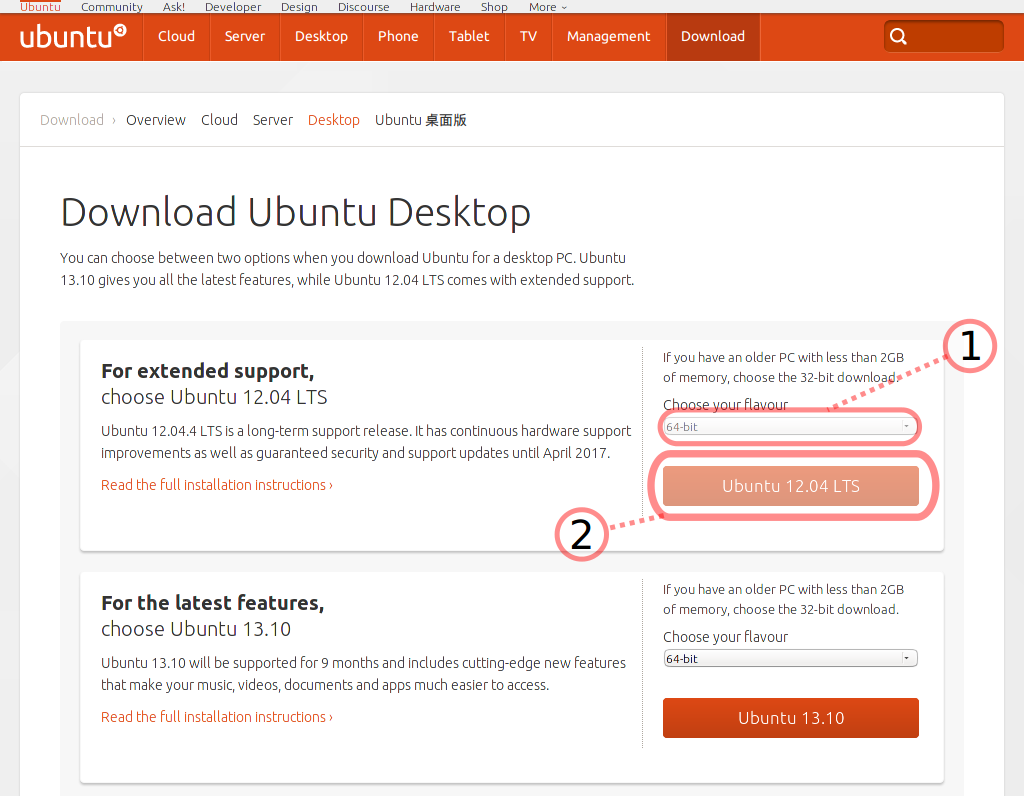
\includegraphics[width=\linewidth]{images/instalacja_pobieranie_obrazu.png}
\end{center}

Pierwszym etapem instalacji systemu jest pobranie instalatora. W tym celu udaj się na stronę \href{http://www.ubuntu.com/download/desktop}{ubuntu.com} i z górnego paska wybierz \textcolor{ubuntu_orange}{Download} a następnie \textcolor{ubuntu_orange}{Desktop}
\begin{enumerate}[label=\protect\circled{\arabic*}]
\item To pole pozwali ci wybrać pomiędzy 32- a 64-bitową wersją systemu. Domyślnie wybrana jest opcja 64 bitowa.
\item Kliknij na ten przycisk aby przejść dalej.
\end{enumerate}

Na kolejnym ekranie będziesz mieć możliwość przekazania dotacji na rzecz Ubuntu. W tym momencie nas to nie interesuje. Przesuń stronę w dół i kliknij na \textcolor{ubuntu_orange}{Not now, take me to the download}. Zostaniesz przeniesiony na kolejną stronę, a po kilku sekundach rozpocznie się pobieranie obrazu systemu.

Jeżeli twój komputer został wyprodukowany nie dawnej niż 5 lat temu, wersja 64-bitowa będzie na pewno odpowiednia. Jeżeli masz mniej niż 2 GB RAM-u, wybierz wariant 32-bitowy. Niezależnie od tego jaką wersję wybierzesz, i tak będziesz mieć dostęp do takiego samego zestawu oprogramowania. Wariant 64-bitowy jest lepiej dopasowany do nowoczesnych systemów, jeżeli jednak masz jakiekolwiek wątpliwości, wybierz wersję 32-bitową. Będzie ona działać także na 64-bitowym komputerze, choć nie będzie wykorzystywać wszystkich jego możliwości.
Jeżeli twoja płyta główna kontrolowana jest przez UEFI, musisz wybrać system 64-bitowy.
Linki do pobierania bezpośredniego:
\begin{itemize}
\item \href{http://www.ubuntu.com/start-download?distro=desktop&bits=64&release=lts}{Wersja 64 bitowa (733 megabajtów).}
\item \href{http://www.ubuntu.com/start-download?distro=desktop&bits=32&release=lts}{Wersja 32 bitowa (731 megabajtów).}
\end{itemize}
	\subsection{Nagrywanie pobranego obrazu}
		\label{nagrywanie_obrazu}
Po zakończeniu pobierania obrazu instalatora należy nagrać go na zewnętrzny nośnik i uruchomić komputer z tego nośnika. Najlepszym rozwiązaniem jest użycie klucza USB (pendrive'a), gdyż obrazy instalacyjne Ubuntu są zbyt duże, aby zmieściły się na typowych krążkach CD o pojemności 700 MB. Weź jednak pod uwagę, że nie wszystkie komputery potrafią startować z klucza USB. Jeżeli twój komputer nie pozwala na wykonanie takiej operacji, będziesz musiał użyć płyty DVD lub karty (micro)SD.
\subsubsection{System Windows, nagrywanie na pendrive'a}
\begin{wrapfigure}[5]{r}{0.5\textwidth}
	\vspace{-10pt}
	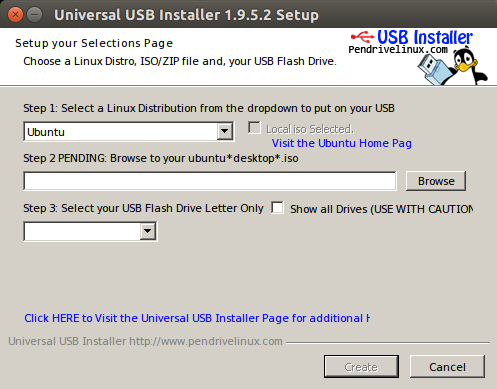
\includegraphics[width=\linewidth]{images/instalacja_nagrywanie_obrazu.png}
\end{wrapfigure}

Jeżeli chcesz użyć pendrive'a jako nośnika instalacyjnego, upewnij się, że ma on przynajmniej 1 GB pojemności (w przeciwnym wypadku instalator się tam po prostu nie zmieści). Jeżeli masz już przygotowany pendrive, wykonaj po kolei następujące kroki:
\begin{enumerate}[label=\protect\circled{\arabic*}]
\item Pobierz program \href{http://www.pendrivelinux.com/downloads/Universal-USB-Installer/Universal-USB-Installer-1.9.5.2.exe}{Universal USB Installer}.
\item Uruchom pobrany plik.
\item Zaakceptuj umowę licencyjną.
\item Podłącz do komputera pendrive, który ma być użyty jako nośnik.
\item Z tej listy wybierz Ubuntu.
\item Kliknij na przycisk \textcolor{ubuntu_orange}{Browse} i wskaż pobrany wcześniej obraz instalatora Ubuntu.
\item Z tej listy wybierz podłączony wcześniej pendrive.\\
\textbf{UWAGA: Wszystkie dane na nim zostaną skasowane!}
\item Kliknij przycisk \textcolor{ubuntu_orange}{Create}.
\item Poczekaj na zakończenie operacji.
\end{enumerate}
\clearpage
\subsubsection{System Windows 7/8, nagrywanie na płytę DVD}
%TODO zweryfikować, czy Windows 8 też to ma
\begin{wrapfigure}[10]{r}{0.5\textwidth}
	\vspace{-10pt}
	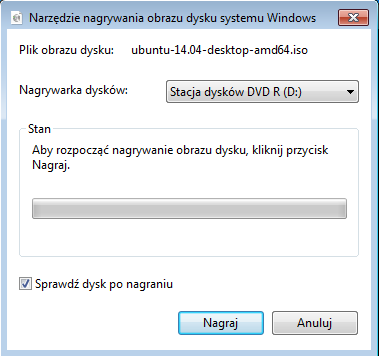
\includegraphics[width=\linewidth]{images/instalacja_nagrywanie_obrazu_DVD.png}
\end{wrapfigure}

Systemy operacyjne Windows 7 i 8 mają wbudowane narzędzie do wypalania plików .iso na płytach. Kliknij prawym przyciskiem myszy na pobrany obraz instalatora Ubuntu, wybierz opcję \textcolor{ubuntu_orange}{Otwórz w} a następnie \textcolor{ubuntu_orange}{Windows Disc Image Burner}.
%TODO jak to się po polsku nazywa?
\begin{enumerate}[label=\protect\circled{\arabic*}]
\item Z tej listy wybierz swoją nagrywarkę.
\item Włóż do wybranego napędu czystą płytę DVD.
\item Upewnij się, że zaznaczone jest pole \textcolor{ubuntu_orange}{Zweryfikuj dysk po nagraniu}.
\item Kliknij przycisk \textcolor{ubuntu_orange}{Nagraj}.
\end{enumerate}

%Pusta przestrzeń, żeby obrazy z sekcji powyżej i poniżej nie wchodziły na siebie.
\vspace{1cm}

\subsubsection{System Windows XP i inne starsze wersje, nagrywanie na płytę DVD}
\begin{wrapfigure}[10]{r}{0.5\linewidth}
	\vspace{-10pt}
	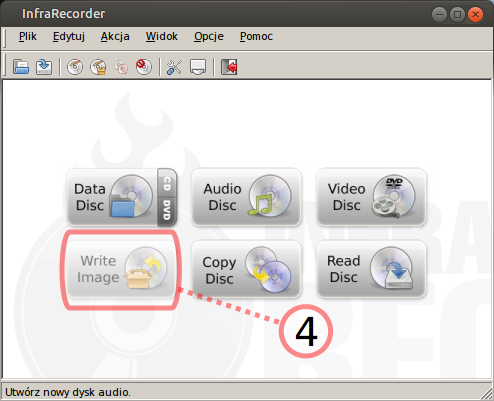
\includegraphics[width=\linewidth]{images/instalacja_nagrywanie_obrazu_DVD_winXP.png}
\end{wrapfigure}

Starsze wersje systemu Windows nie mają wbudowanej możliwości nagrywania płyt DVD. Potrzebne będzie do tego osobne narzędzie służące do wypalania płyt. Obsługa tych programów jest bardzo podobna: należy wybrać opcję \textcolor{ubuntu_orange}{Nagrywanie obrazu na płytę}. Koniecznie nagrywaj z wykorzystaniem tej opcji, gdyż inne (np. ,,Nagrywanie płyty z danymi'' lub ,,Tworzenie kopii zapasowej'') utworzą dysk, którego nie będzie można użyć do uruchomienia komputera. Dla przykładu posłużymy się programem Infra Recorder.

\begin{enumerate}[label=\protect\circled{\arabic*}]
\item Pobierz i zainstaluj program \href{http://infrarecorder.org/?page_id=5}{Infra Recorder}.
\item Uruchom zainstalowany przed momentem program.
\item Włóż czystą płytę DVD do nagrywarki.
\item W programie Infra Recorder wybierz opcję \textcolor{ubuntu_orange}{Write Image}.
\item Wybierz pobrany wcześniej obraz instalatora systemu Ubuntu.
\item Kliknij przycisk \textcolor{ubuntu_orange}{OK}.
\end{enumerate}

\subsubsection{System Linux, nagrywanie na pendrive'a}
\begin{wrapfigure}{r}{0.5\textwidth}
	\vspace{-10pt}
	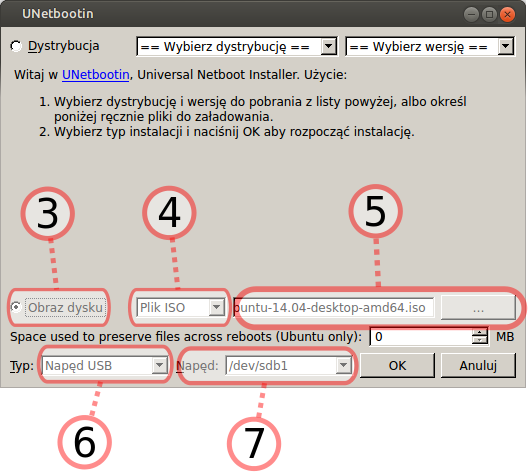
\includegraphics[width=\linewidth]{images/instalacja_nagrywanie_obrazu_linux.png}
\end{wrapfigure}

W systemach operacyjnych Linux do nagrywania obrazu na pendrive'a najlepiej posłużyć się programem \textcolor{ubuntu_orange}{UNetbootin}, dostępnym w większości popularnych dystrybucji. UNetbootin rozpakuje pobrany obraz instalatora (plik .iso) bezpośrednio na pendrive'a, a następnie zainstaluje na nim program rozruchowy.

Sposób uruchomienia instalatora (opisywany w dalszej części tego przewodnika) nieco się różni, jeżeli użyłes programu UNetbootin. Po uruchomieniu komputera z tak przygotowanego pendrive'a, wyświetlony zostanie niebieski ekran z opcjami instalacji, ale bez możliwości wyboru języka. Nazwy opcji są identyczne z tymi opisanymi w rozdziale \ref{instalacja_uruchomienie_uefi}: Uruchomienie instalatora UEFI. Różnią się one tylko szatą graficzną.
\begin{enumerate}[label=\protect\circled{\arabic*}]
\item Zainstaluj UNetBootIn korzystając ze swojego menadżera pakietów.
\item Uruchom zainstalowany przed momentem program.
\item Zaznacz pole Obraz dysku.
\item Z menu wybierz Plik ISO.
\item W tym polu podaj ścieżkę do pobranego wcześniej obrazu instalatora Ubuntu. Wciśnij przycisk oznaczony trzema kropkami (“\ldots”) i wskaż plik.
\item W tym menu wybierz Napęd USB.
\item Z tego menu wybierz podłączony wcześniej pendrive.\\
\textbf{UWAGA: Wszystkie dane znajdujące się na tym nośniku zostaną skasowane!}
\item Kliknij przycisk \textcolor{ubuntu_orange}{OK}, aby rozpocząć nagrywanie.
\end{enumerate}

\subsubsection{System Linux, nagrywanie na DVD}
%TODO potrzebny obrazek z włożoną płytą DVD i wybranym obrazem ubuntu 14.04
\begin{wrapfigure}{l}{0.5\textwidth}
	\vspace{-10pt}
	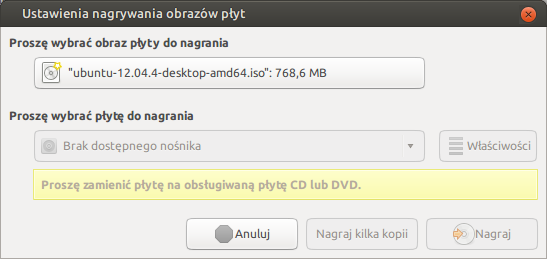
\includegraphics[width=\linewidth]{images/instalacja_nagrywanie_obrazu_linux_DVD.png}
\end{wrapfigure}

Aby nagrać obraz na płytę DVD, potrzebujesz odpowiedniego programu. W tym przykładzie posłużymy się dostępną w większości dystrybucji nagrywarką Brasero. Kliknij prawym przyciskiem myszy na pobrany wcześniej obraz instalatora Ubuntu i wybierz
\menu{{Otwórz w \ldots}>{Brasero}}. W otwartym oknie zostaniesz poproszony o włożenie czystej płyty DVD. Zrób to, a następnie kliknij przycisk \textcolor{ubuntu_orange}{Nagraj}.

\end{document}